\documentclass{beamer}
\usepackage{graphicx}
\usepackage{amsmath}
\usepackage{listings}
\usepackage{xcolor}
\usepackage{helvet}

% Define colors for code and presentation theme
\definecolor{codegreen}{rgb}{0,0.6,0}
\definecolor{codegray}{rgb}{0.5,0.5,0.5}
\definecolor{codepurple}{rgb}{0.58,0,0.82}
\definecolor{themecolor}{RGB}{45, 62, 80}

% Setup for code blocks
\lstset{
  language=Python,
  basicstyle=\footnotesize\ttfamily,
  keywordstyle=\color{blue},
  commentstyle=\color{codegreen},
  stringstyle=\color{codepurple},
  numbers=left,
  numberstyle=\tiny\color{codegray},
  breaklines=true,
  showspaces=false,
  showstringspaces=false,
  showtabs=false,
  tabsize=4
}

% Beamer theme
\usetheme{Madrid}
\usecolortheme[named=themecolor]{structure}

% Title information
\title{\textbf{Regression Analysis of Used Car Prices}}
\author{Tancredi Bosi}
\institute{Alma Mater Studiorum Bologna}
\date{\today}

\setbeamertemplate{footline}{%
  \leavevmode%
  \hbox{%
    \begin{beamercolorbox}[wd=.3\paperwidth,ht=2.25ex,dp=1ex,leftskip=2ex]{author in head/foot}%
      Tancredi Bosi%
    \end{beamercolorbox}%
    \begin{beamercolorbox}[wd=.4\paperwidth,ht=2.25ex,dp=1ex,center]{title in head/foot}%
      Regression Analysis of Used Car Prices%
    \end{beamercolorbox}%
    \begin{beamercolorbox}[wd=.3\paperwidth,ht=2.25ex,dp=1ex,right]{date in head/foot}%
      \insertframenumber{} / \inserttotalframenumber%
    \end{beamercolorbox}%
  }%
  \vskip0pt%
}


\begin{document}

% Title slide
\begin{frame}
    \titlepage
\end{frame}

% Outline slide
\begin{frame}{Outline}
    \tableofcontents
\end{frame}

% Problem Definition
\section{Problem Definition}
\begin{frame}{Problem Definition}
    \begin{itemize}
        \item Predicting the price of used cars based on various features
        \item Data sourced from \href{https://www.kaggle.com/competitions/playground-series-s4e9}{Kaggle competition}
    \end{itemize}
    \begin{figure}
        \centering
        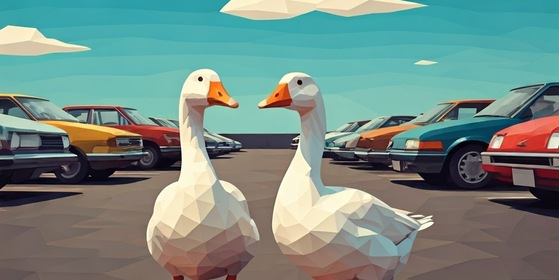
\includegraphics[width=0.6\linewidth]{images/kaggle_car_price_main_image.png}
        \caption{Kaggle competition image}
    \end{figure}
\end{frame}

% Dataset Overview
\section{Dataset}
\begin{frame}{Dataset Overview}
\begin{itemize}
    \item Dataset details:
        \begin{itemize}
            \item 188,533 rows, 12 features, and 1 target column (price)
            \item Numerical features: \textit{id, model\_year, milage}
            \item Categorical features: \textit{brand, model, fuel\_type, engine, transmission, ext\_col, int\_col, accident, clean\_title}
        \end{itemize}
        \begin{figure}
            \centering
            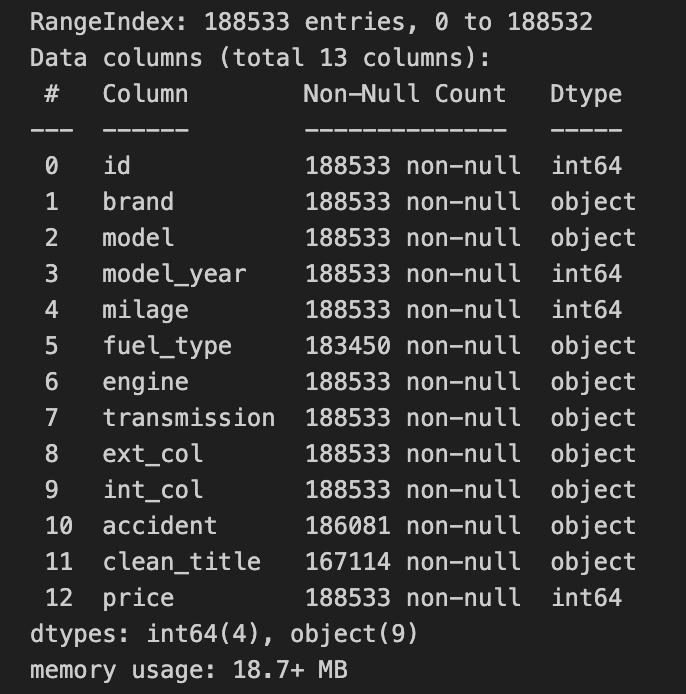
\includegraphics[width=0.3\linewidth]{images/dataset_info.png}
            \caption{Dataset info}
            \label{fig:enter-label}
        \end{figure}
\end{itemize}
\end{frame}

% Data Exploration
\begin{frame}{Data Exploration}
    \begin{figure}
        \centering
        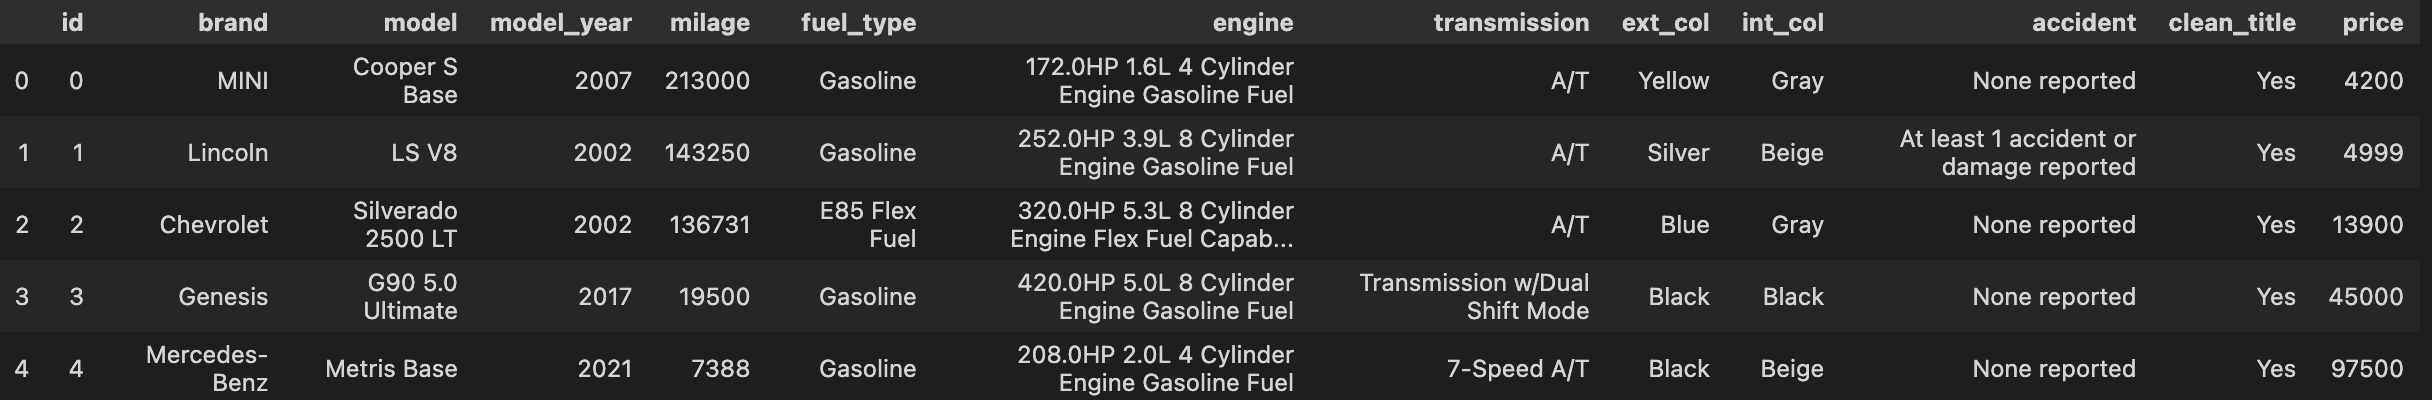
\includegraphics[width=1\linewidth]{images/data_head_initial.png}
        \caption{Head of the dataset}
        \label{fig:enter-label}
    \end{figure}
    We can already see that:
    \begin{itemize}
        \item "id" column can be dropped as it refers only to the index of the car.
        \item "brand" and "model" columns seem to have a lot of different unique values.
        \item "engine" column has useful and different information abridged in one string.
        \item "ext\_col" and "int\_col" columns are the colors of the cars and they may be not so useful.
    \end{itemize}
\end{frame}

% Data Visualization
\section{Data Visualization}
\begin{frame}{Data Visualization}
    \begin{itemize}
        \item Price distribution by brand:
            \begin{figure}
                \centering
                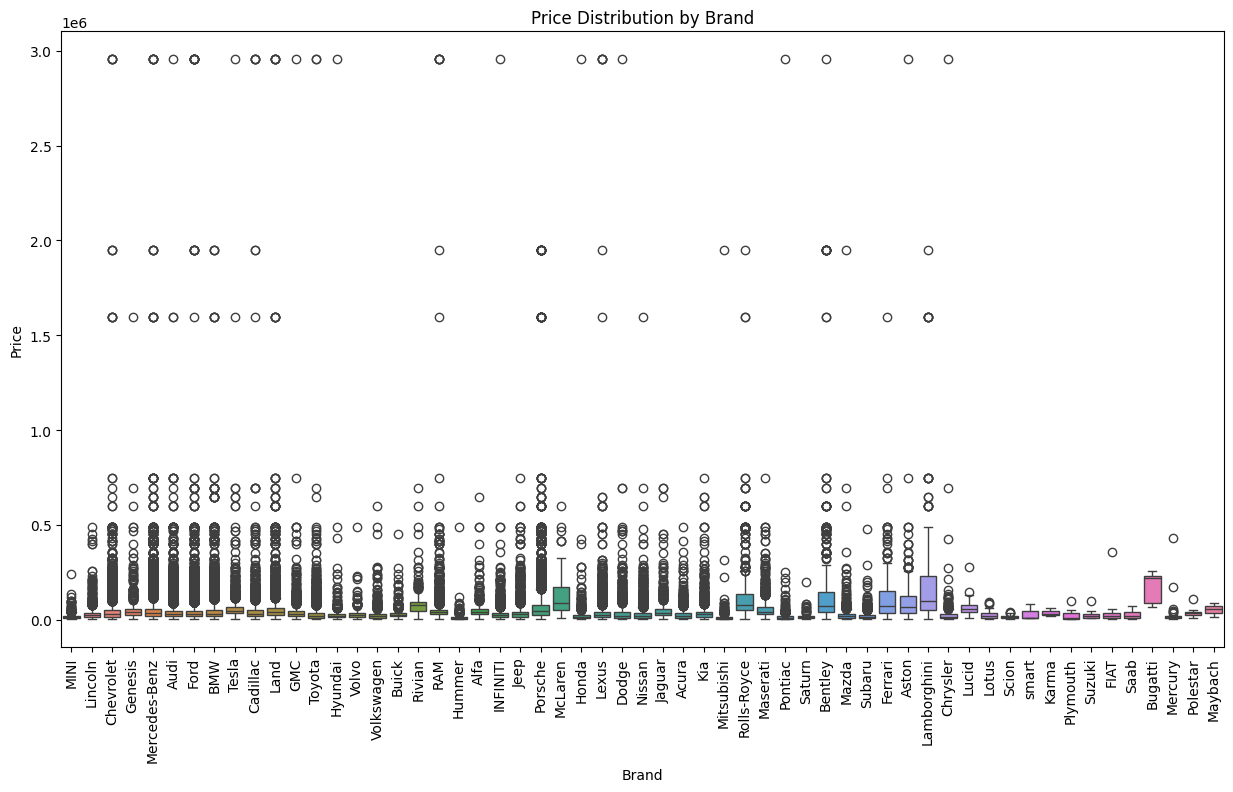
\includegraphics[width=1\linewidth]{images/boxplot_price_distribution_by_brand.png}
            \end{figure}
    \end{itemize}
\end{frame}

\begin{frame}{Data Visualization}
    \begin{itemize}
        \item Average price by model year:
            \begin{figure}
                \centering
                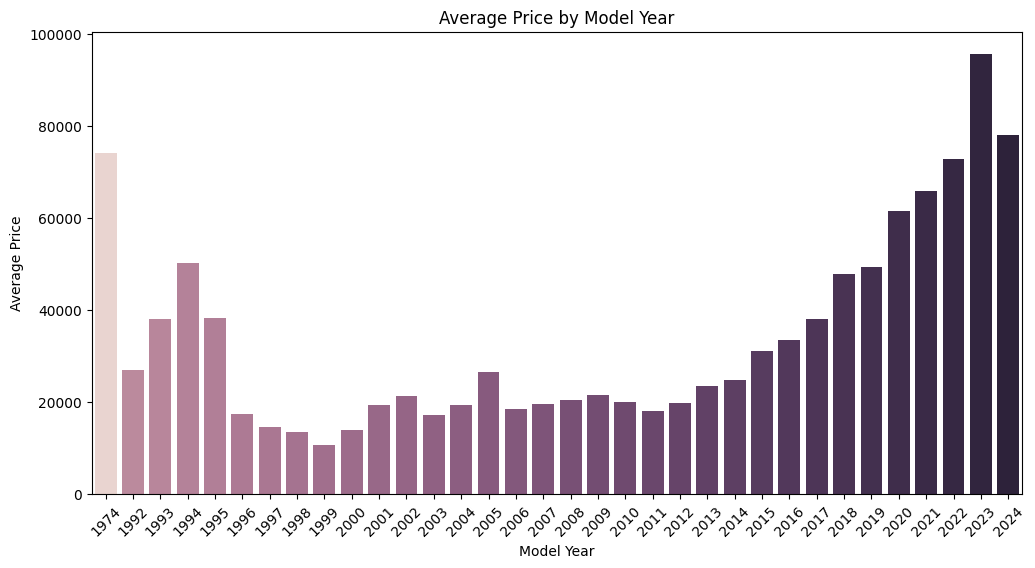
\includegraphics[width=1\linewidth]{images/avg_price_by_model_year.png}
            \end{figure}
    \end{itemize}
\end{frame}

% Data Preprocessing
\section{Data Preprocessing}
\begin{frame}{Data Preprocessing}
    \begin{itemize}
        \item Remove outliers
        \begin{figure}
            \centering
            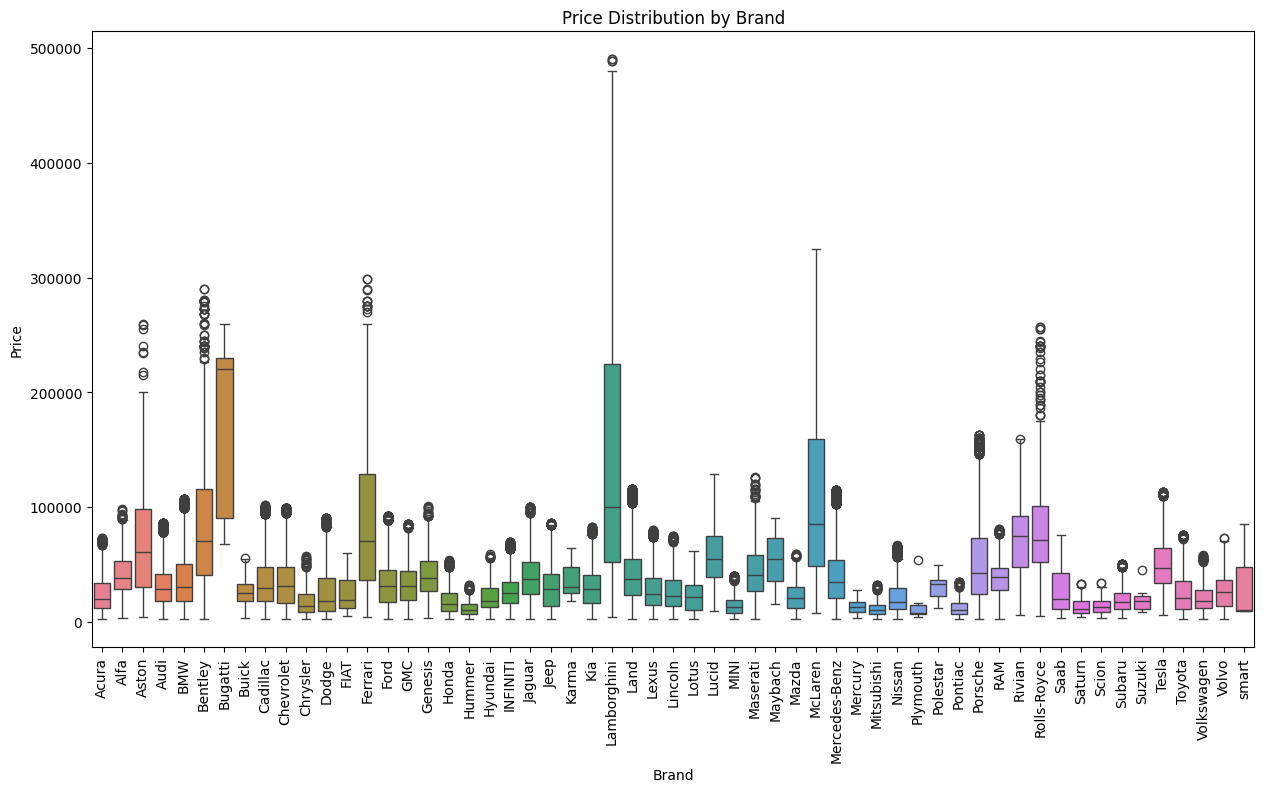
\includegraphics[width=0.5\linewidth]{images/remove_outliers_boxplot_price_by_brand.png}
            \label{fig:enter-label}
        \end{figure}
        \item Extract \textit{vehicle\_age} as \(vehicle\_age = 2024 - model\_year\)
        \item Extract \textit{HP, engine\_size} and \textit{cylinders} from \textit{engine}
        \item Extract \textit{speed} and \textit{transmission\_type} from \textit{transmission}
        \item Extract \textit{luxury\_brand} from \textit{brand} and \textit{model\_category} from \textit{model}, to reduce the unique values in the two columns
    \end{itemize}
\end{frame}

\begin{frame}{Data Preprocessing}
    \begin{itemize}
        \item Fill missing values with 'Unknown' or 0
        \item Remove \textit{id, ext\_col} and \textit{int\_col} columns
        \item Scale \textit{milage, vehicle\_age, HP} and \textit{engine\_size} with \textbf{RobustScaler()}
        \item Enconde:
            \begin{itemize}
                \item \textit{accident} in 0/1
                \item \textit{speed} in numerical values
                \item \textit{transmission\_type} in 0/1
                \item \textit{clean\_title} in 0/1
                \item \textit{fuel\_type, luxury\_brand} and \textit{model\_category} with One-Hot Encoding
            \end{itemize}
    \end{itemize}
    The final features for each sample are:
    \begin{figure}
            \centering
            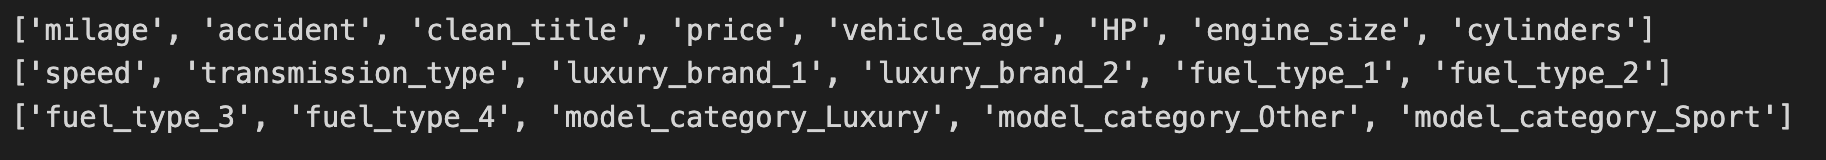
\includegraphics[width=1\linewidth]{images/POST-PROCESS_DATA_HEAD.png}
            \label{fig:enter-label}
    \end{figure}
\end{frame}

% Model Selection
\section{Model Selection}
\begin{frame}{Model Selection}
    \begin{itemize}
        \item Dataset division: 80\% training set, 20\% test set.
        \item Measures in output: Train-RMSE, Test-RMSE
        \item Models considered:
            \begin{itemize}
                \item Ridge Regressor (least squares with l2 regularization)
                \item Random Forest Regressor with standard hyperparameters
                \item Support Vector Regressor
                \item Random Forest Regressor with Grid Seach
                \item MLP Regressor
                \item AdaBoost Regressor with Decision Tree
                \item AdaBoost Regressor with Random Forest Regressor
            \end{itemize}
    \end{itemize}
\end{frame}

% Results
\section{Model Results}
\begin{frame}{Ridge Regressor}
\textbf{Ridge()} performance:
        \begin{itemize}
            \item Train RMSE: 19192
            \item Test RMSE: 18877
        \end{itemize}
    \begin{figure}
        \centering
        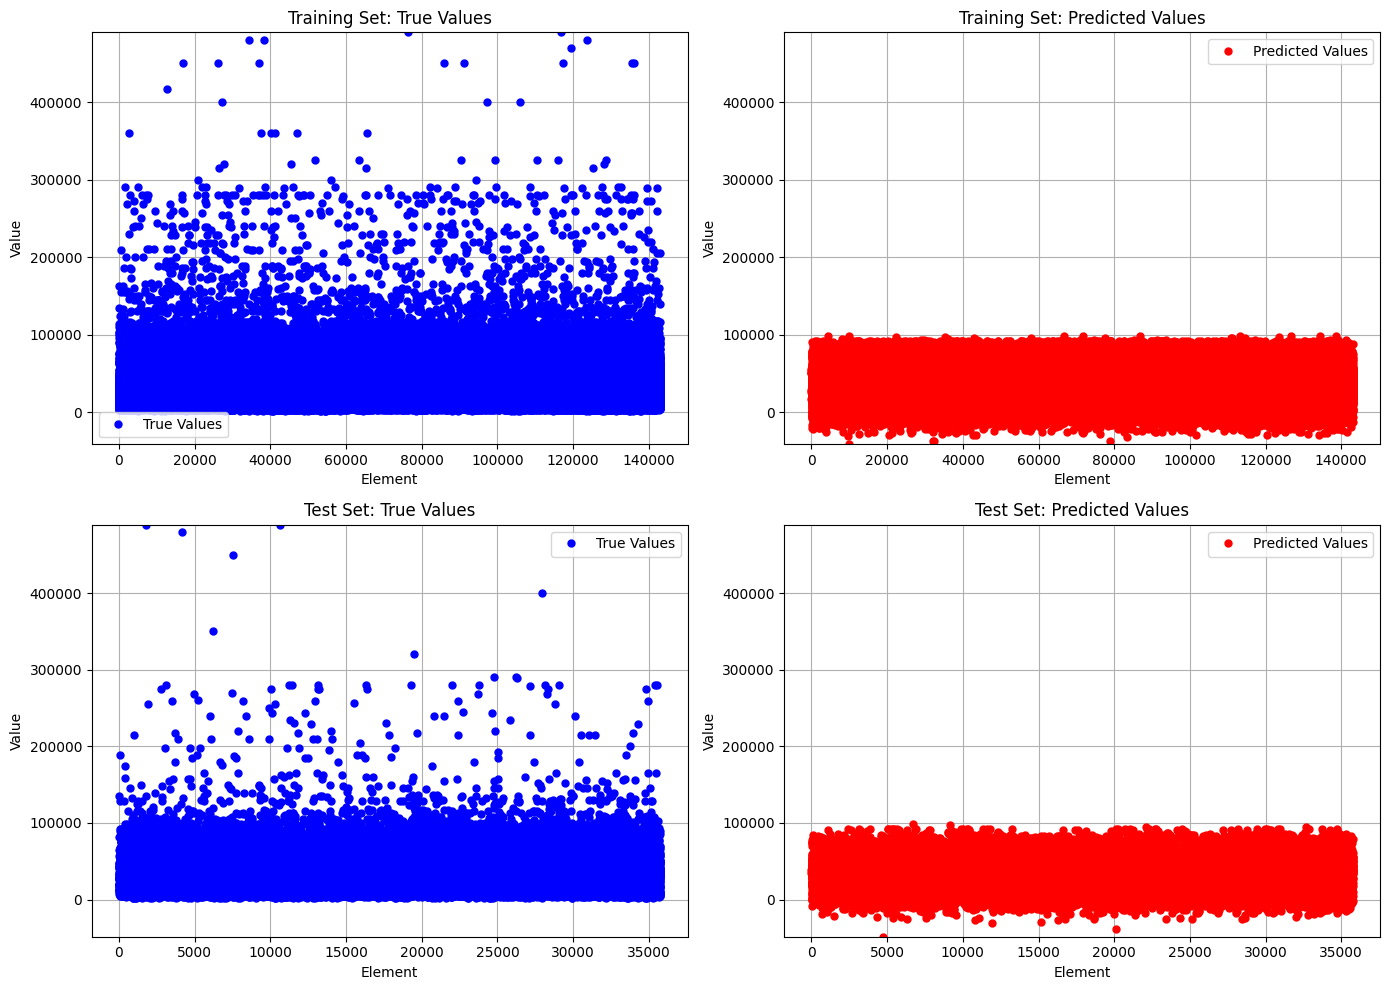
\includegraphics[width=0.65\textwidth]{images/ridge_plot2.png}
    \end{figure}
\end{frame}

\begin{frame}{Default Random Forest Regressor}
\textbf{RandomForestRegressor()} performance:
        \begin{itemize}
            \item Train RMSE: 8134
            \item Test RMSE: 17625
        \end{itemize}
    \begin{figure}
        \centering
        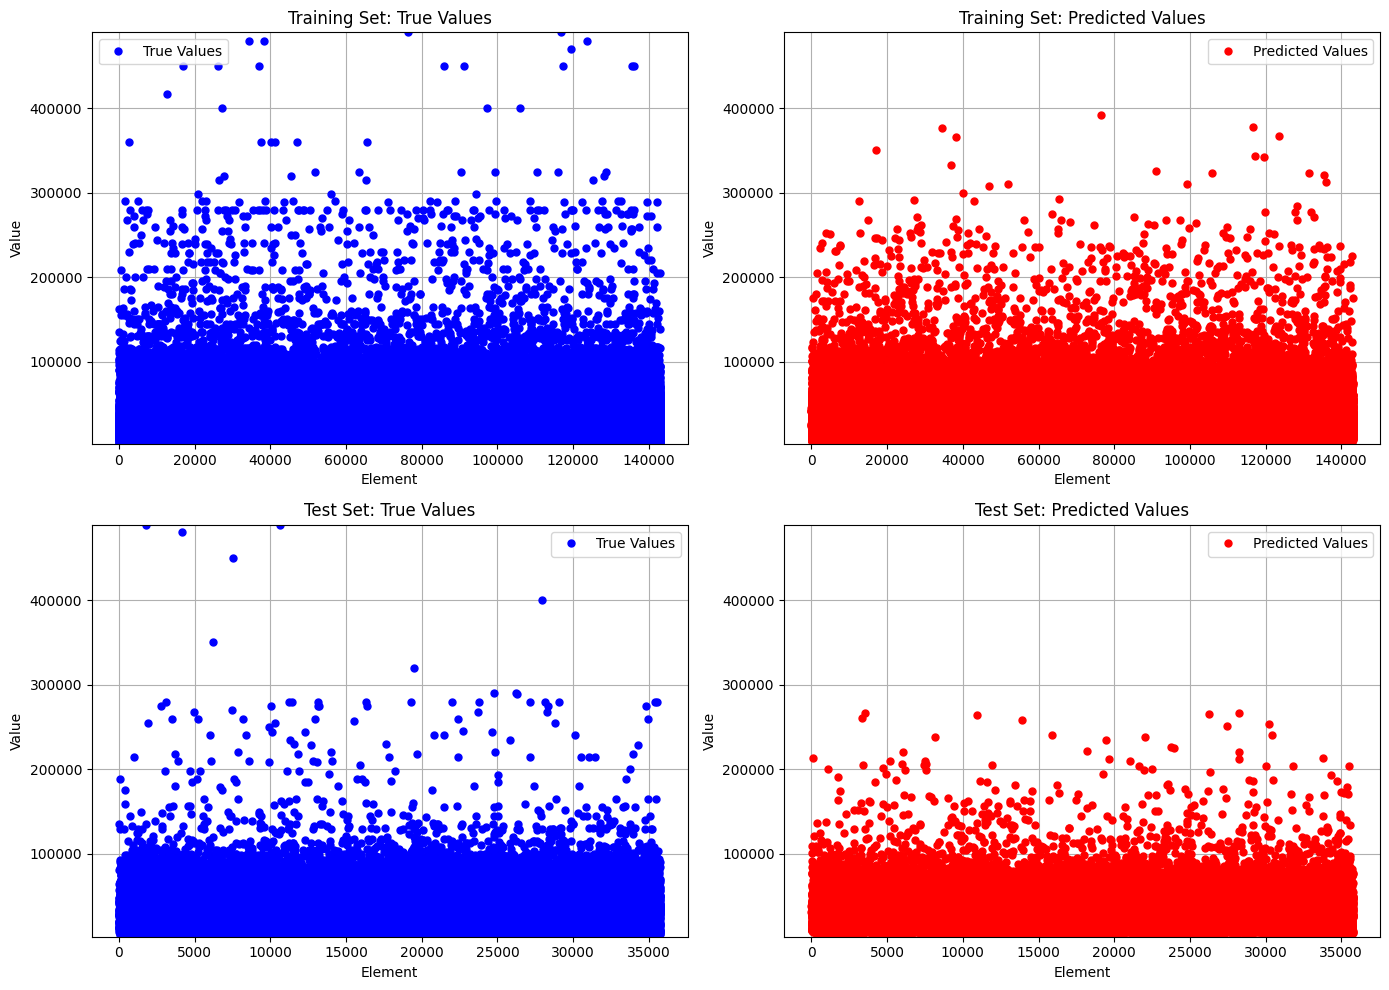
\includegraphics[width=0.65\textwidth]{images/RFR_default_plot2.png}
    \end{figure}
\end{frame}

\begin{frame}{Grid Search Random Forest Regressor}
\textbf{RandomForestRegressor(}n\_estimators=100, max\_depth= 12, min\_samples\_split= 14, min\_samples\_leaf= 3\textbf{)} performance:
        \begin{itemize}
            \item Train RMSE: 15129
            \item Test RMSE: 16518
        \end{itemize}
    \begin{figure}
        \centering
        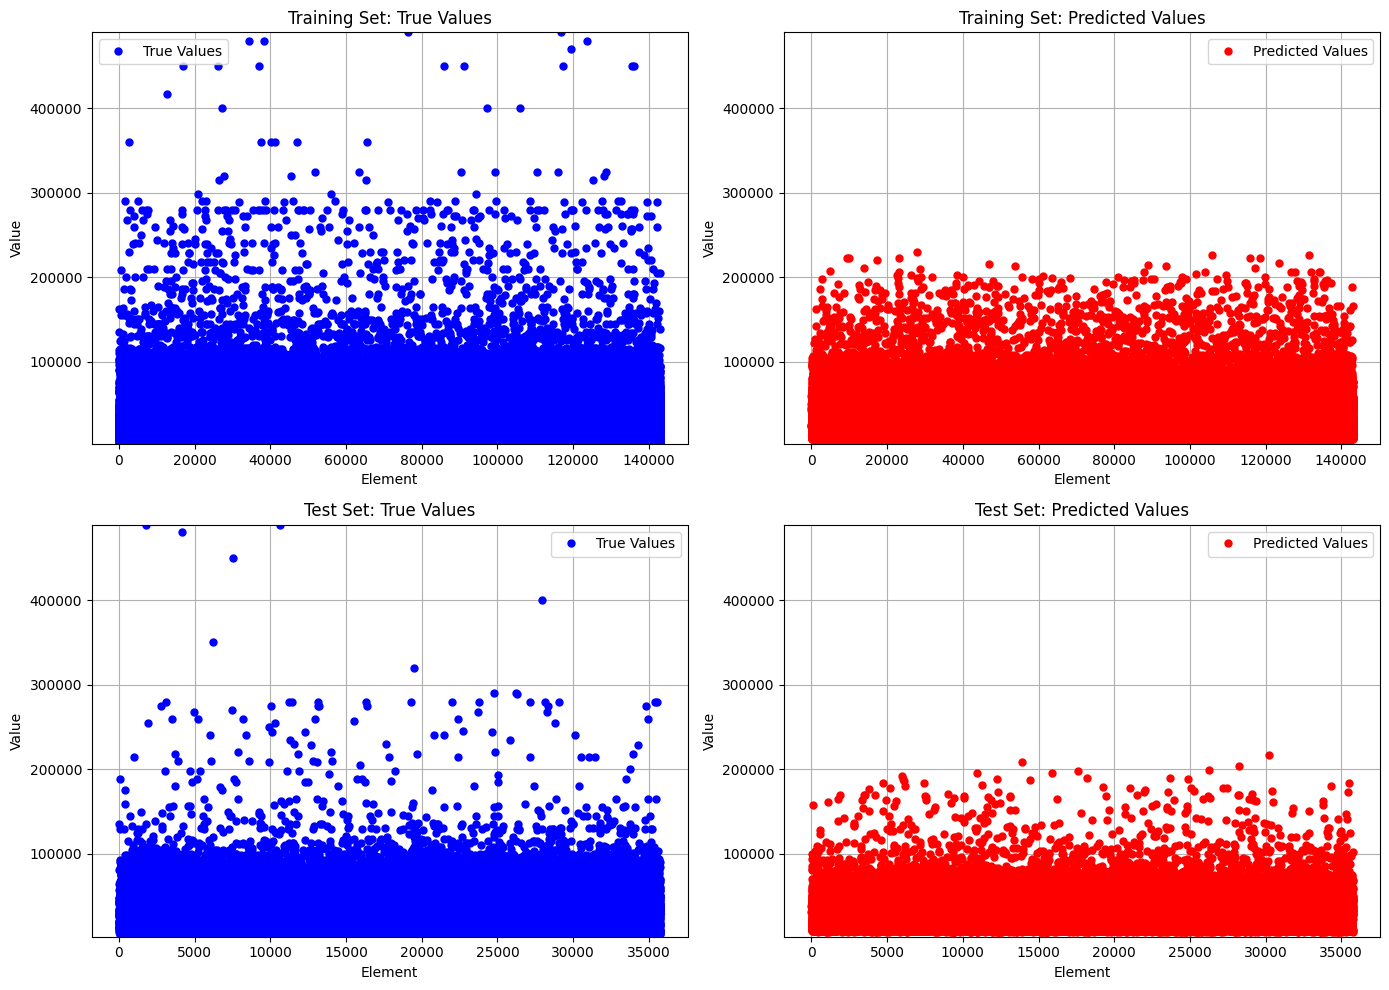
\includegraphics[width=0.65\textwidth]{images/GSRFR_plot2.png}
    \end{figure}
\end{frame}

\begin{frame}{AdaBoost Regressor - DT}
\textbf{AdaBoostRegressor()} performance:
        \begin{itemize}
            \item Train RMSE: 19941
            \item Test RMSE: 19990
        \end{itemize}
    \begin{figure}
        \centering
        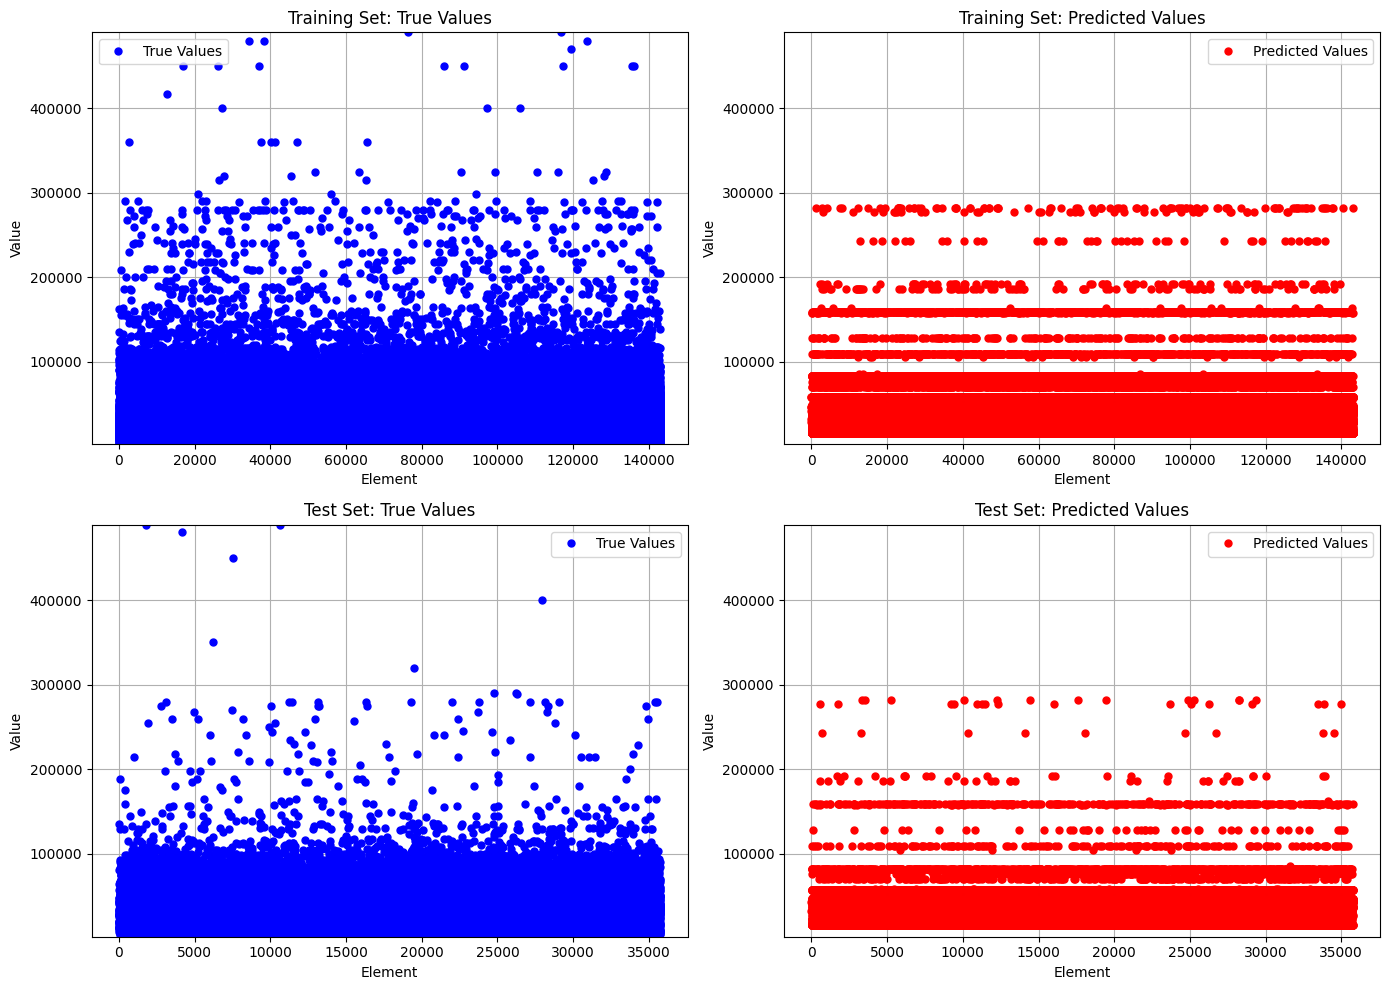
\includegraphics[width=0.65\textwidth]{images/AdaBR_default_plot2.png}
    \end{figure}
\end{frame}

\begin{frame}{AdaBoost Regressor - RF}
\textbf{AdaBoostRegressor(}estimator=RandomForestRegressor()\textbf{)} (with grid-search hyperparameters) performance:
        \begin{itemize}
            \item Train RMSE: 14432
            \item Test RMSE: 16710
        \end{itemize}
    \begin{figure}
        \centering
        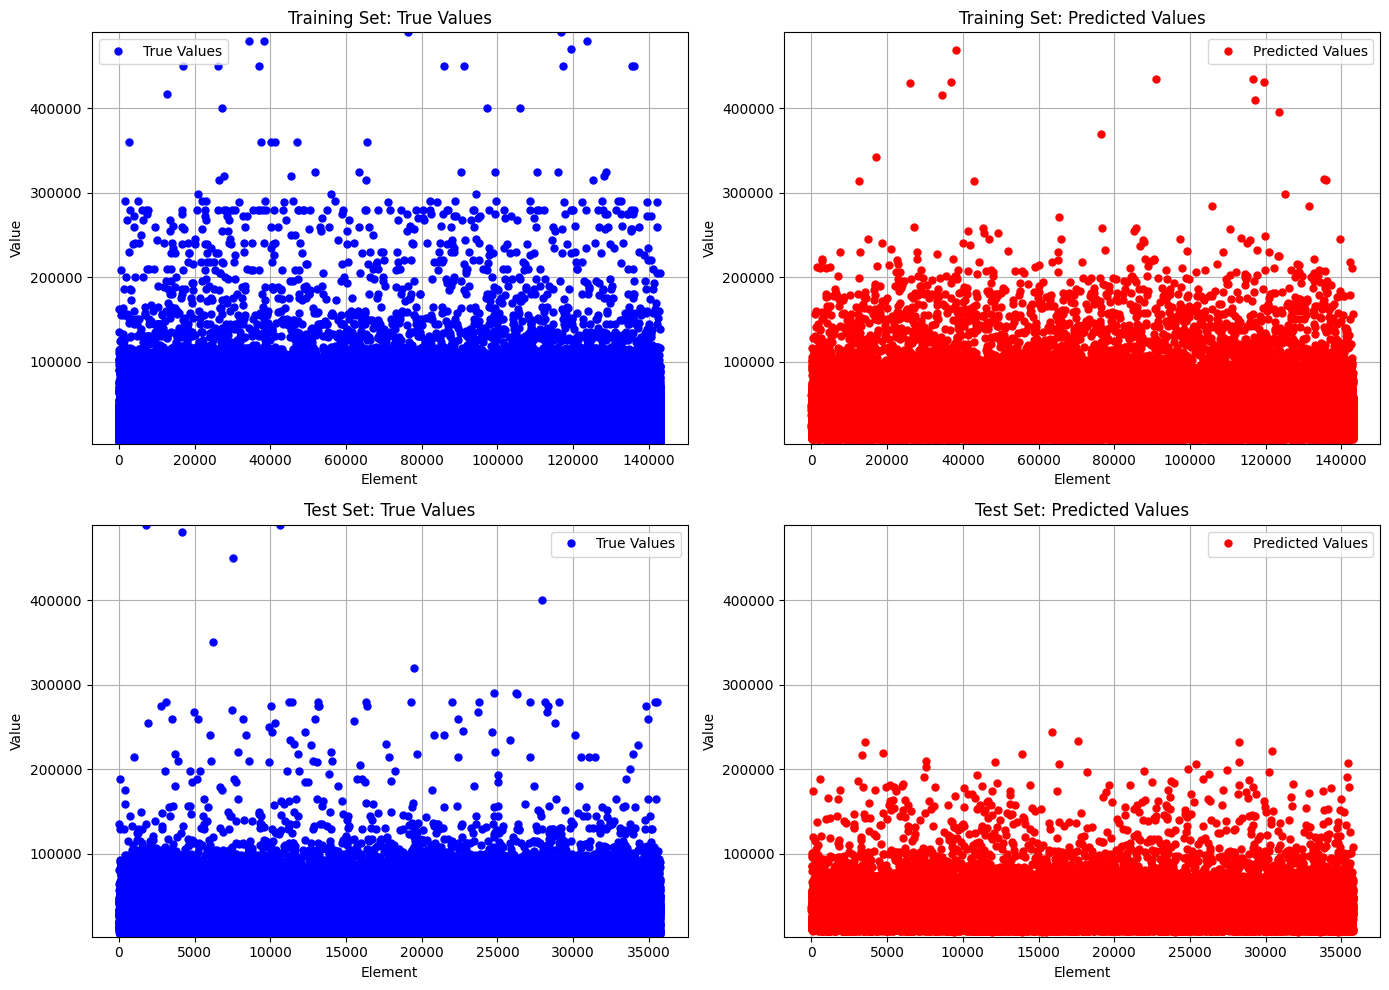
\includegraphics[width=0.65\textwidth]{images/AdaBR_RF_plot2.png}
    \end{figure}
\end{frame}

\begin{frame}{MLP Regressor}
\textbf{MLPRegressor(}hidden\_layer\_sizes=(128, 256, 512, 256, 128), max\_iter=1000, learning\_rate='adaptive'\textbf{)} performance:
        \begin{itemize}
            \item Train RMSE: 14572
            \item Test RMSE: 17955
        \end{itemize}
    \begin{figure}
        \centering
        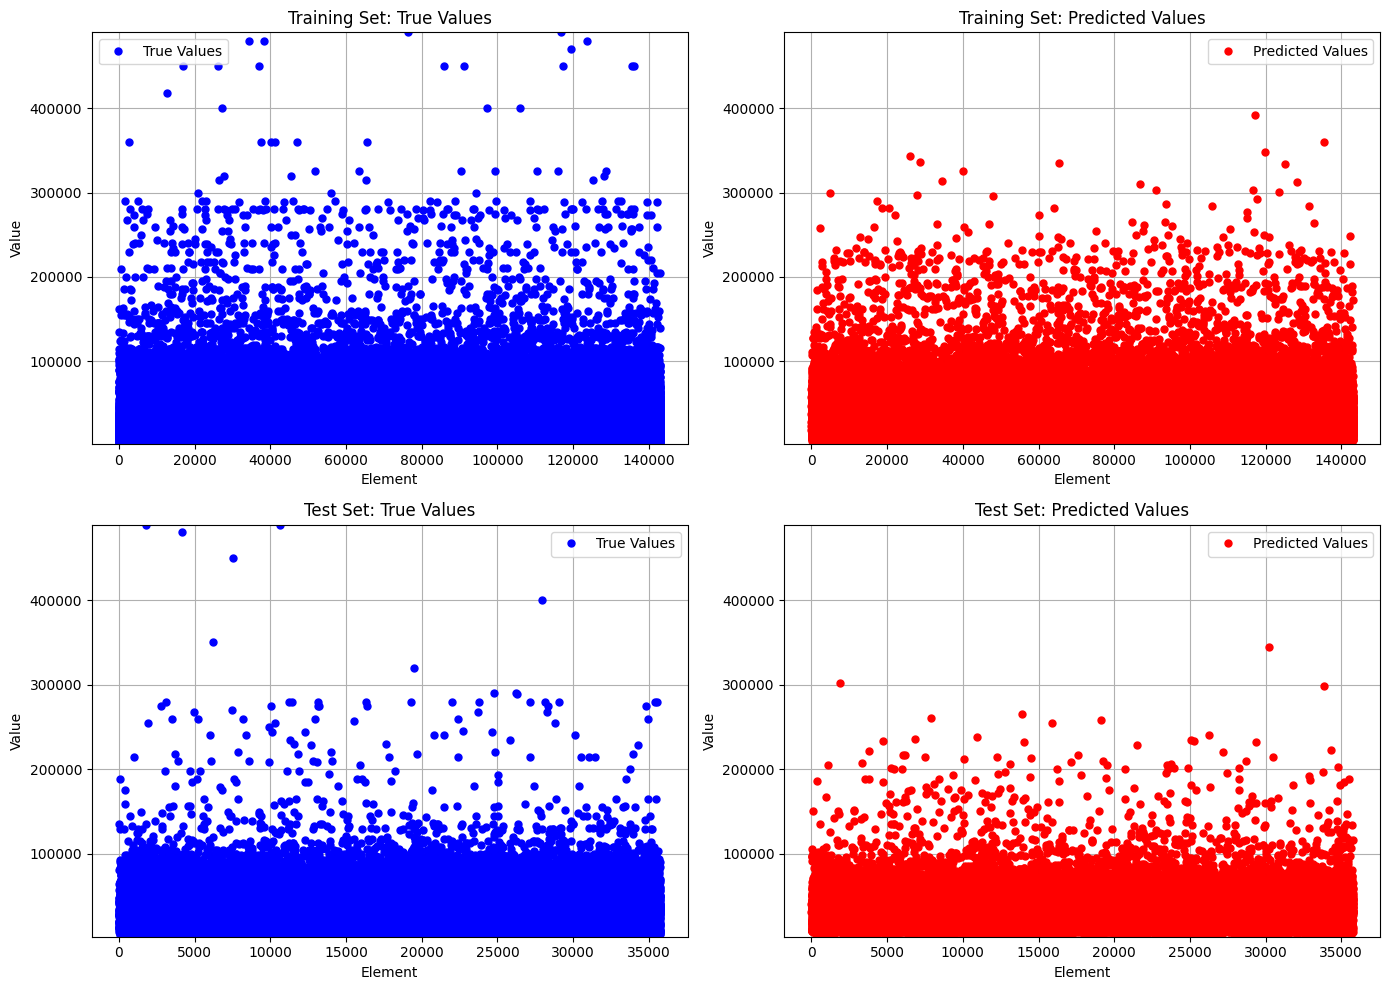
\includegraphics[width=0.65\textwidth]{images/MLPregressor_plot2.png}
    \end{figure}
\end{frame}

% Conclusion
\section{Results Conclusions}
\begin{frame}{Results Conclusions}
Here the models for a comparison:
    \begin{table}[h!]
    \centering
    \renewcommand{\arraystretch}{1.3}
    \setlength{\tabcolsep}{12pt}
    \begin{tabular}{|l|c|c|}
        \hline
        \textbf{Model} & \textbf{Train RMSE} & \textbf{Test RMSE} \\
        \hline
        Ridge Regressor & 19192 & 18877 \\
        Random Forest Regressor & 8134 & 17625 \\
        Random Forest Regressor GS & 15129 & 16518 \\
        Ada Boost Regressor DT & 19941 & 19990 \\
        Ada Boost Regressor RF & 14432 & 16710 \\
        MLP Regressor & 14572 & 17955 \\
        \hline
    \end{tabular}
    \caption{Model performance comparison}
    \end{table}
\end{frame}

\end{document}
